\documentclass{bioinfo}
\copyrightyear{2005}
\pubyear{2005}



%=================== package declaration ===================
\usepackage{algorithm}

% for the CLRS style pseudocode typing
\usepackage{clrscode3e}





\begin{document}
\firstpage{1}

\title[IBD statistics used in demographic inference]{A Simulation-based Approach for Demographic Inference via Identity-by-Descent Haplotype Sharing}
\author[Yang and Hu]{Shuo Yang\,$^{1}$\footnote{to whom correspondence should be addressed} $\ $and Jing Hu\,$^{1}$}
%\author[Yang and Hu\textit{et~al}]{Shuo Yang\,$^{1}$\footnote{to whom correspondence should be addressed} $\ $and Jing Hu\,$^{1}$}
\address{$^{1}$Department of Computer Science, Columbia University, New York, NY 10027, USA}

\history{Received on XXXXX; revised on XXXXX; accepted on XXXXX}

\editor{Associate Editor: XXXXXXX}

\maketitle

\begin{abstract}

\section{Motivation:}
With the fast development of DNA sequencing technology, there is an increasing amount of genomic data ready for deeper analysis. How to interpret these data becomes a challenge for genetic researchers. When the population evolutionary model becomes more realistic but complicated, theories that can precisely explain the data are very difficult to develop even with much mathematical approximation. Thus, computational simulation gives us a novel and more powerful direction for exploring the evolutionary model of these genomic data, or more specifically, demographic inference.

\section{Results:}
In this project, we evaluated a new statistic within the simulation-based framework for demographic inference via Identity-by-Descent (IBD) haplotype sharing. The new statistic which is natural to be used in haplotype imputation, characterizes the average sharing of IBD among samples. We also combined the new statistic with the well-studied IBD length distribution statistic, and demonstrated that simple combination wouldn't improve the precision of the inference. After all, our new approach that utilizes the IBD statistics for demographic inference will work better for recent history inference compared to the traditional site frequency spectrum (SFS) based methods, because long haplotype sharing contains more information about recent population history that shapes the chromosome recombination process. What's more, our project provides a possible model that statistics of genetic data can be used together with computational simulation to explore its novel significance for the study of demographic history.

\section{Availability:}
All source code is available online and free for download at https://github.com/morrisyoung/CompGenome.

\section{Contact:} \href{sy2515@columbia.edu}{sy2515@columbia.edu}
\end{abstract}






\section{Introduction}

Nowadays, population genetics are entering a new era, and the needs for computational simulation are highly strengthened. Complicated genetic phenomena sometimes are possible be described with simple mathematical models. However, it is not simply fulfillable all the time, especially when the demographic model of genetic data is too complicated to be simplified by mathematical approximation. In this case, we cannot use analytical approach to explain the genetic data, instead, a simpler but still effective method will be greatly favored. Bioinformatics researchers then proposed the simulation-based method, for example, the one in~\cite{Excoffier2013} is absolutely an important component in the relevant research.

However, there are two main challenges in this novel approach. The first one is to choose the appropriate statistics for the simulation framework, which, to some extent, will determine the effectiveness of the whole simulation-based approach. And the second one is to find an efficient way for the simulation and inference, which will possibly limit the application of this new approach.

As we have seen in~\cite{Excoffier2013}, site frequency spectrum (SFS) has already been used frequently in such approach. Researchers used SFS in demographic inference to explain the genomic data, and the results demonstrated both accuracy and efficiency especially for very complicated models. Also, the composite likelihood method they used is very flexible in their model, which may be further exploited in other works. However, the SFS based method will dramatically lose its power when we are specifically interested in the recent history from the genetic data. In recent demographic history, long haplotype sharing provides more information, and the variance of SFS is not as statistically significant from short time as it is from long evolution history. Enlightened by this, we plan to use the long haplotype sharing between two reportedly unrelated individuals among a cohort, formally defined as Identity-by-Descent (IBD), with its rich statistics in our simulation framework, to explain the recent history of the genomic data.

Based on some well-established theories that has been commonly used to describe the evolution models in population genetics, such as sequential Markov coalescent (SMC) and SMC' (see~\cite{McVean2005} and~\cite{Marjoram2006}), we can easily simulate the genetic data under various population models with high confidence in their accuracy. Lots of downstream statistics can then be extracted using computational approaches. Our main task, at this stage, is to integrate our simulation and statistical inference works with the existing simulators, so that to evaluate the effectiveness of new statistics used in our demographic inference. And finally, we are going to build a framework with appropriate computational power requirements, that dedicates for simulation-based demographic inference of recent population history.





\section{Approach}

We will start from very simple population models -- constant population size model and the bottleneck population model (Figure~\ref{fig:model}). They are simple enough for a good start for our exploratory research. And our second model -- the bottleneck model is especially supposed to be consistent with what really happened in recent history in certain human populations. The parameter we are interested in the constant population size model is the effective population size $N$ (or $N_{e}$ in some traditional literature). In the bottleneck model, we are interested in the following parameters:

\begin{enumerate}
\item $NA$: ancient population size;
\item $NC$: current population size;
\item $TB$: time to bottleneck event;
\item $NB$: bottleneck population size; or $T$: bottleneck duration;
\item $\frac{T}{NB}$: bottleneck strength
\end{enumerate}

For these parameters, we set the default values in our testing as: $NA=10000$, $NC=10000$, $TB=30$, $NB=200$, $T=10$.

\begin{figure}[h]
\centerline{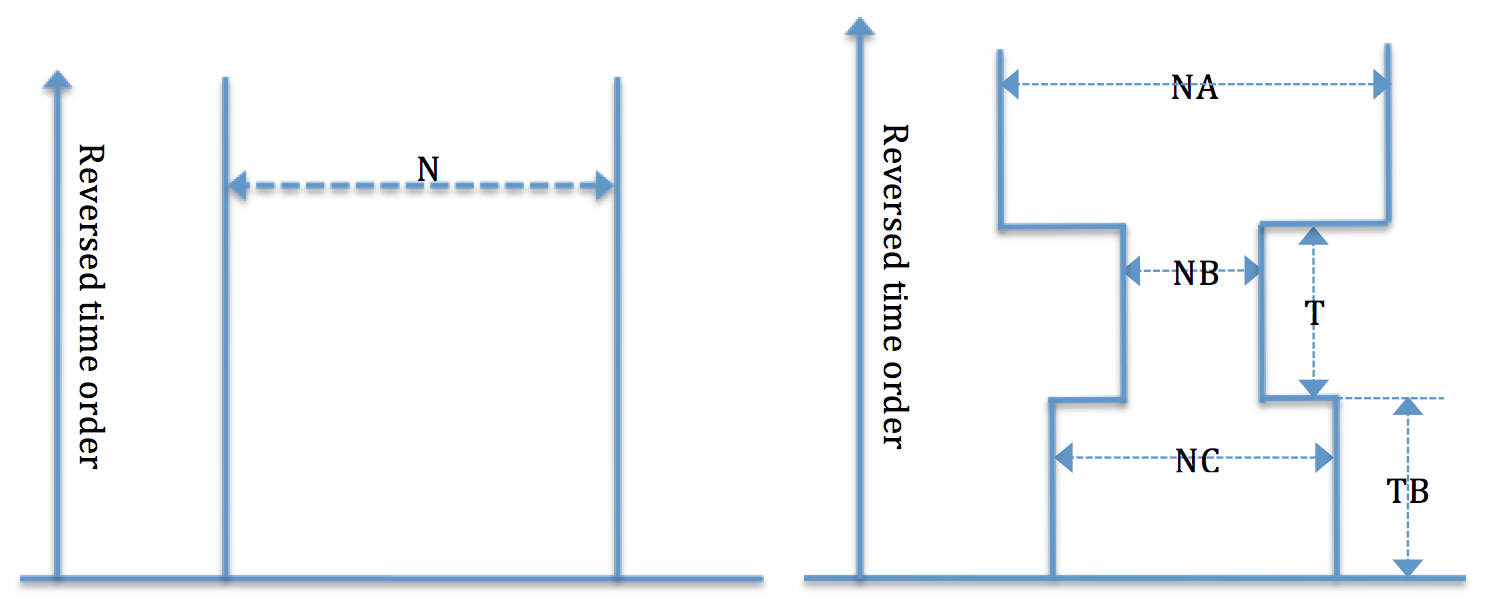
\includegraphics[width=240pt, height=100pt]{model}}
\caption{Two models to be evaluated. The left one is the simple constant population size model, which is not very realistic in practice. The right one is the bottleneck model, which is consistent with true human population history for some populations.}\label{fig:model}
\end{figure}

In all of these models, the preliminary works are based on IBD segment number distribution (results not shown), and we will now use a new statistic -- average IBD sharing statistic, in our inference framework, and try to compare the new results with those from old statistic. The explanation of this statistic is from~\ref{fig:newstats}~\cite{Carmi2014}. This new statistic origins from the genome sequencing. Intuitively, the more sequenced individuals from a population we have in hand, the larger proportion of cohort-sharing IBD segments will present, indicating that the average fraction of the genome of one individual that can be imputed via the sequenced chromosomes increases. Though it's a natural statistic for genome sequencing, this statistic actually gives us a more thorough and clearer description of the cohort-sharing properties of IBD segments, and how it is shaped by historical events. Therefore it is worth to be exploited for demographic analysis of population genetics.


\begin{figure}[h]
\centerline{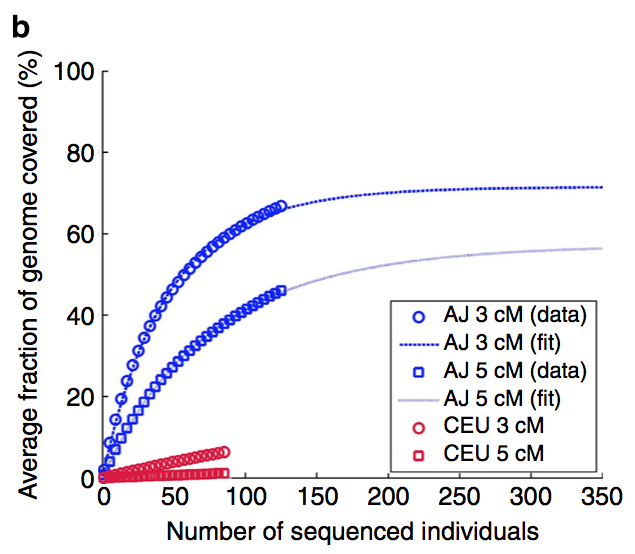
\includegraphics[width=160pt, height=140pt]{NewStats}}
\caption{The average sharing of IBD with increased number of reference genomes within a cohort.}\label{fig:newstats}
\end{figure}

To get these statistic data, we will try the simulation methods, because we don't have exact theories of the statistics (especially the new one) for these models. And it is why we call our methods simulation-based methods.





\begin{methods}
\section{Methods}

We will use \textit{fastsimcoal2} (\cite{Excoffier2013}) to simulate the genomes according to different population parameters. We will also use \textit{IBDdetection} (\cite{Yang2015}) to extract the ground-truth IBD segments from simulated Ancestry Recombination Graph (ARG). The IBD segments used in the demographic analysis should be ground-truth, as they will act as the reference genomes, and that's why we directly extract IBD segments from ARG other than the sequence data. These software are enough for evaluation purpose, and we actually didn't practically infer the parameters (that's less meaningful than the evaluation first of all).

We will use the procedure in Algorithm~\ref{algo:newstats} to generate the new statistic with simulations. Specially, $\Theta$ is the population parameters we use to generate the samples and the IBD statistics. It should contain the value of $N$, $NA$, $NC$, $NB$, $T$ and $TB$. $n$ is the sample size in the simulation. The output of the procedure is the new statistic: average fraction of IBD cohort-sharing corresponding to the case of $x$ reference genomes are sequenced, where $x$ is equal to $[5,10,...,n]$.

\begin{algorithm}
\caption{IBD average sharing statistic generating}
\label{algo:newstats}
\vspace{-0.32cm}  % this vspace should be legal, because it's inside another module (algorithm box)
\begin{codebox}
\Procname{$\proc{NewStats}(\Theta, n)$}
\li	$Stats=\{5:0, 10:0, 15:0, ... , n:0\}$
\li	$Simu=20$\Comment{$20$ simulations are used to average}
\li	$Iter=50$\Comment{$50$ samplings are used to average}
\li \For $i=1,2,...,Simu$
\li	\Do	\textit{fastsimcoal2}($\Theta$)
\li		\For $j=1,2,...,Iter$
\li		\Do \For $k=5,10,15,...,n$\Comment{where statistics are picked}
\li			\Do randomly sample $1$ genome, as $g$
\li				randomly sample $k$ genomes, as $G$
\li				$IBDdetection$($g$), $IBDdetection$($G$)
\li				$f=$ fraction of co-sharing between $g$ and $G$
\li				$Stats[k]+=f$
			\End
		\End
	\End
\li	$Stats=\frac{Stats}{Simu \times Iter}$
\li	return $Stats$
\end{codebox}
\vspace{-0.35cm}  % this vspace should be legal, because it's inside another module (algorithm box)
\end{algorithm}

Specially, to average the statistics we get from simulation, we run $20$ simulations with the specified population parameters. Also, for each $k$ (the number of reference genomes that are sequenced), we randomly sample $50$ times (for both the target genome and these $k$ genomes). With this strategy, we hope to get the statistics as what they actually are.

Also, to get the distance between two statistics, we will utilize Algorithm~\ref{algo:distance} (squared distance). In this study, we will draw the distance curve (or surface if two parameters are estimated jointly), to evaluate whether the minimum distance between guessed parameter value and the true parameter value exactly happens in the true value. If that is the case, we can optimize along the distance curve (or surface) to retrieve the true parameter value, and that's what we call effective demographic inference.

\begin{algorithm}
\caption{distance calculating from IBD cohort-sharing}
\label{algo:distance}
\vspace{-0.32cm}  % this vspace should be legal, because it's inside another module (algorithm box)
\begin{codebox}
\Procname{$\proc{Distance}(Stats_1, Stats_2)$}
\li	$dis = 0$
\li	\For $k=5,10,15,...,n$
\li	\Do	$dis += (Stats_1[k] - Stats_2[k])^2$
	\End
\li	return $dis$
\end{codebox}
\vspace{-0.35cm}  % this vspace should be legal, because it's inside another module (algorithm box)
\end{algorithm}

In the final stage, after comparing the new statistic with the old one, we will try to combine them to see whether it will help. As the new statistic provides us extra and independent information about the population evolution (but not necessarily perfect information), combining it with the old one to make them contribute roughly equally may characterize the population history better. We will discuss later about how to combine them in an empirical but effective way.

\end{methods}




\section{Results}

We show that, with the new average IBD sharing statistic, we evaluated all parameters with either distance curve or joint distance surface. We also show the combined distance curve when we tried to integrate the two statistics at the same time. We worked on the constant size population model first, and then the bottleneck model.

\subsection{Constant population size model}

Figure~\ref{fig:dis_N} shows different statistics of average IBD sharing under different population size $N$. The trend of the distributions across different value of $N$ tells us that the inference is feasible for the chosen parameter. Then we show the distance curve for different $N$ compared to the true value, here $N=5000$, in Figure~\ref{fig:like_N}. This parameter is also tested to be feasible with old statistic -- IBD number distribution (data not shown).

\begin{figure}[h]
\centerline{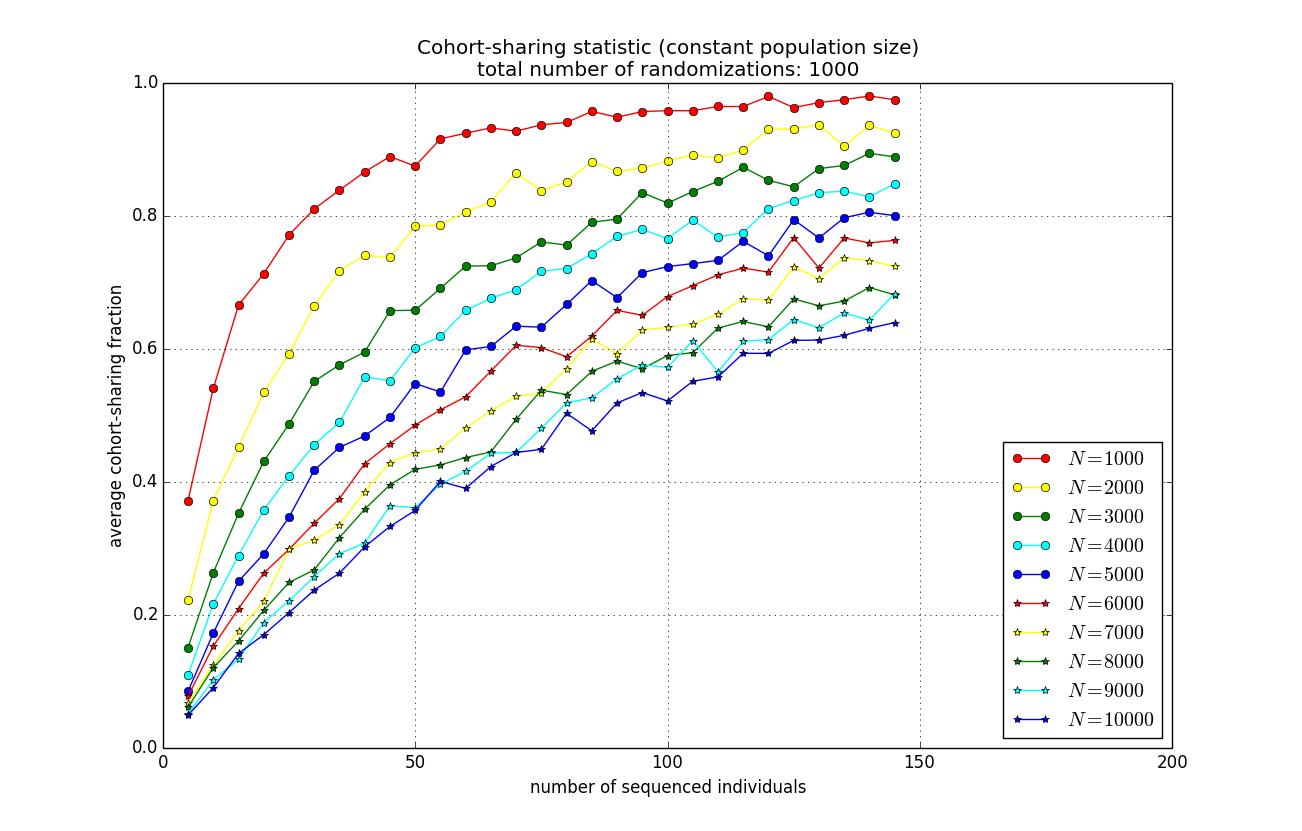
\includegraphics[width=290pt, height=200pt]{dis_N.png}}
\caption{Different statistics of average IBD sharing across different $N$.}\label{fig:dis_N}
\end{figure}

\begin{figure}[h]
\centerline{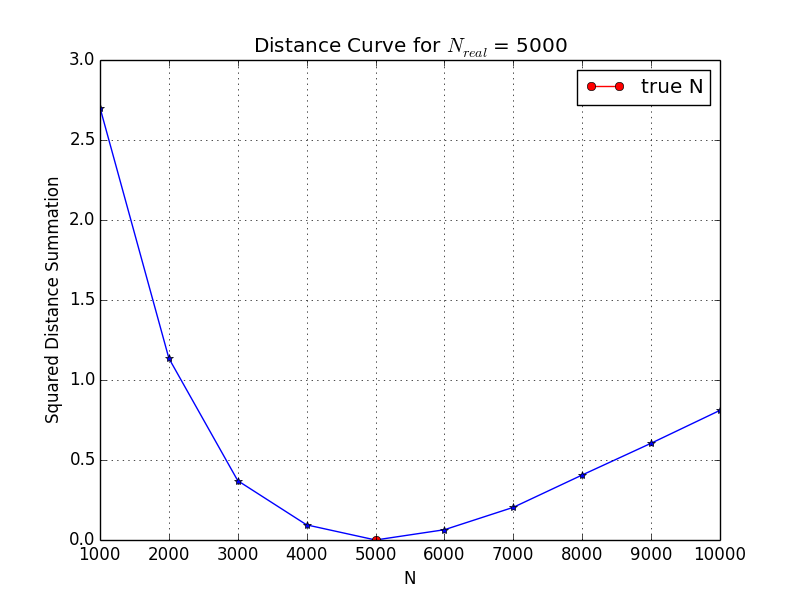
\includegraphics[width=280pt, height=200pt]{like_N.png}}
\caption{The corresponding distance curve for Figure~\protect\ref{fig:dis_N} if true parameter is $N=5000$. In this case, minimum distance happens exactly in the true parameter value.}\label{fig:like_N}
\end{figure}



\subsection{Bottleneck model}

Now we will test the bottleneck model, for which we are interested in $NA$, $NC$, $NB$, $T$ and $TB$, or certain combinations of them. To evaluating one of these parameters, we will consider all other parameters as their \textquotedblleft true" value\footnote{the value used in the model to generate the \textquotedblleft observed" samples.}. If we evaluate two parameters jointly, we will consider all other parameters as their \textquotedblleft true" value, and only the two joint parameters are unknow.

$NA$ and $NC$ are the two parameters we are always interested in, as population size always (but not all the time) greatly affect the evolutionary history of the population. In Figure~\ref{fig:dis_NA} and~\ref{fig:dis_NC}, we show their distance curve, which seems not promising. This observation matches our expectation. In the bottleneck model, the IBD sharing information of current genomes seems to be highly dependent on the bottleneck event itself, but not the ancient/current population size. So we hold more interests to analyze the bottleneck event with this IBD sharing information. The same results are achieved for the old statistic IBD segment number distribution (data not shown).

\begin{figure}[h]
\centerline{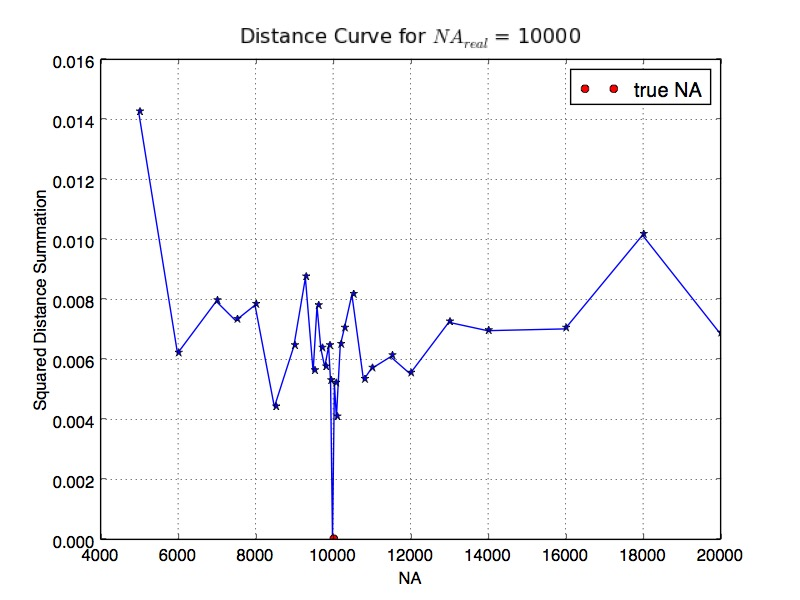
\includegraphics[width=280pt, height=200pt]{like_NA.jpg}}
\caption{The distance curve for $NA$ if true parameter is $NA=10000$. In this case, minimum distance doesn't necessarily happen in the true parameter value, as this curve is not convex. Indeed, it's not even smooth at all.}\label{fig:dis_NA}
\end{figure}

\begin{figure}[h]
\centerline{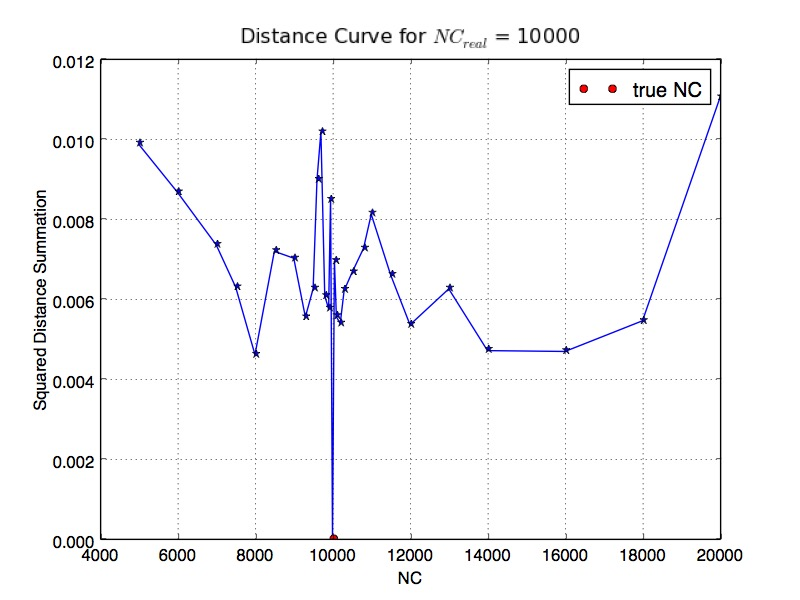
\includegraphics[width=280pt, height=200pt]{like_NC.jpg}}
\caption{The distance curve for $NC$ if true parameter is $NC=10000$. In this case, minimum distance doesn't necessarily happen in the true parameter value, as this curve is not convex. Indeed, it's not even smooth at all. This is similar to the curve of $NA$.}\label{fig:dis_NC}
\end{figure}

We are now interested in the bottleneck event itself. We start from $TB$, which is the time point when this bottleneck event first appeared back in time. From the Figure~\ref{fig:dis_TB}, we can see this parameter is also unfeasible to estimate. This is very different from the results of IBD segment number distribution statistic, in which $TB$ is feasible to estimate.

\begin{figure}[h]
\centerline{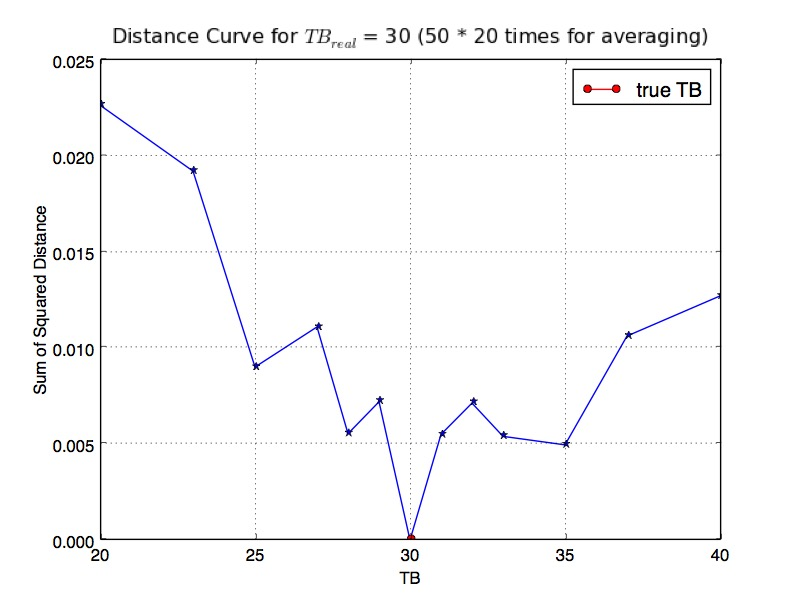
\includegraphics[width=280pt, height=200pt]{like_TB.jpg}}
\caption{The distance curve for $TB$ if true parameter is $TB=30$. In this case, minimum distance doesn't necessarily happen in the true parameter value, as this curve is not convex. Indeed, it's not even smooth at all.}\label{fig:dis_TB}
\end{figure}

However, according to our results of IBD segment number statistic, such imperfect $TB$ won't affect the other two parameters in the bottleneck event -- $NB$ and $T$, so we will show the joint distance curve (surface) for $NB$ with $TB$, and $T$ with $TB$ next, in Figure~\ref{fig:dis_NBTB} and~\ref{fig:dis_TBT}. These two parameters also show a same trend that, without perfect information of $TB$, we can still estimate them, if we fix other parameters (including $NB$ and $T$) as their true value.

\begin{figure}[h]
\centerline{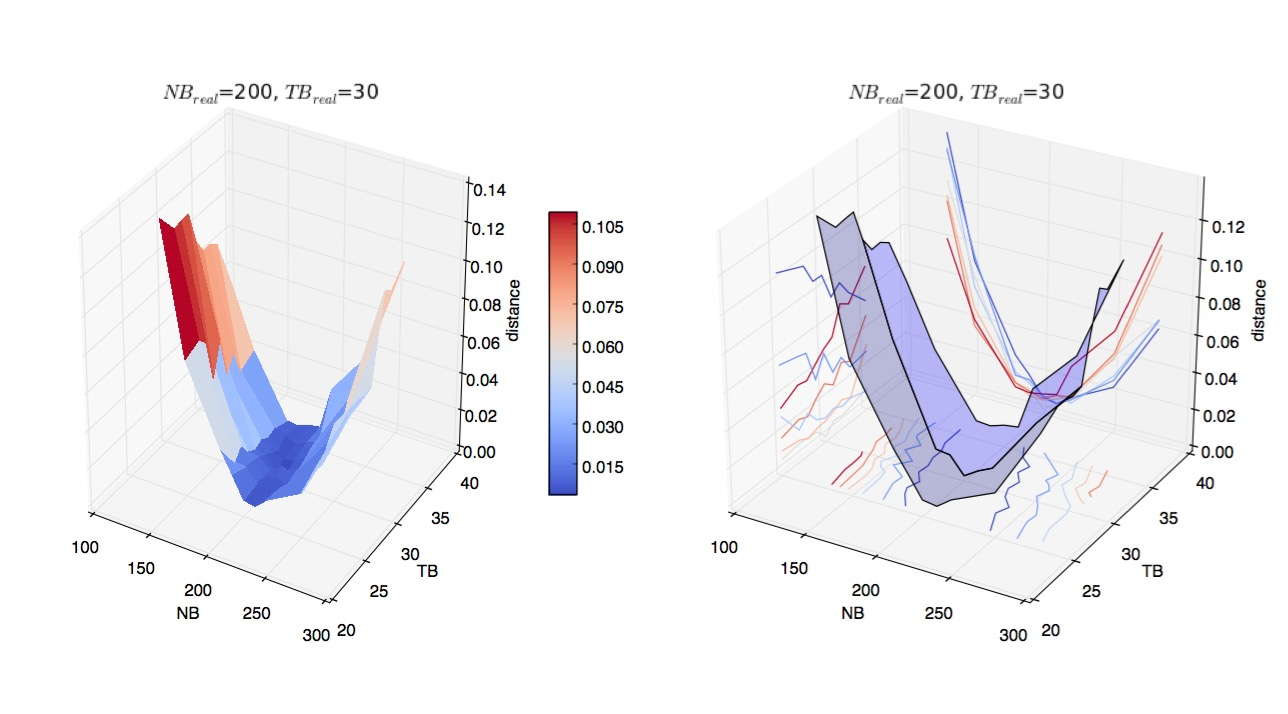
\includegraphics[width=270pt, height=150pt]{like_NBTB.jpg}}
\caption{The joint distance surface for $NB$ and $TB$ if true parameter is $NB=200,TB=30$. We can see from the surface that, $TB$-dimension is always noisy (not estimatable), while $NB$-dimension is always good enough to estimate no matter what $TB$ is.}\label{fig:dis_NBTB}
\end{figure}

\begin{figure}[h]
\centerline{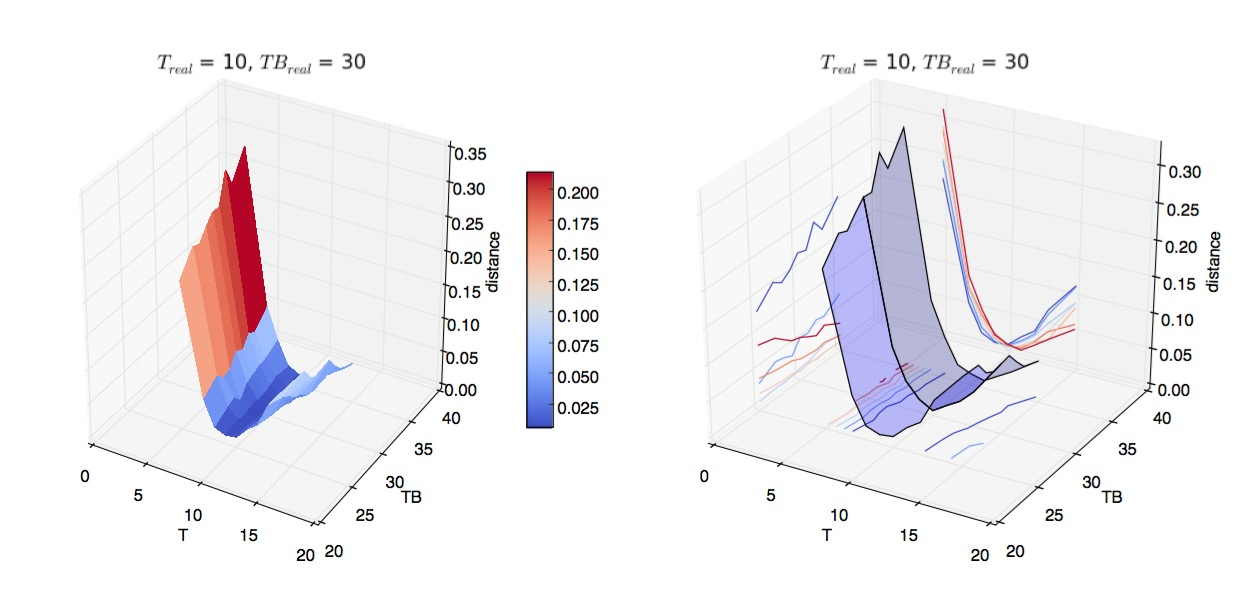
\includegraphics[width=270pt, height=150pt]{like_TBT.jpg}}
\caption{The joint distance surface for $T$ and $TB$ if true parameter is $T=10,TB=30$. We can see from the surface that, $TB$-dimension is always noisy (not estimatable), while $T$-dimension is always good enough to estimate no matter what $TB$ is.}\label{fig:dis_TBT}
\end{figure}

In the above evaluation, whenever we evaluate $NB$ or $T$ with $TB$, we fix $T$ or $NB$ (the other parameters) as their true value. Now we will jointly estimate this two parameters -- $NB$ and $T$. In Figure~\ref{fig:dis_NBT}, it is, again, similar to what we observed from the IBD segment number distribution. There is a diagonal in the joint parameter space, which seems to achieve the global minimum value all the time. It indicates that, under the current model, the separate true value of $NB$ and $T$ are not able to be determined, while their ratio can be.

\begin{figure}[h]
\centerline{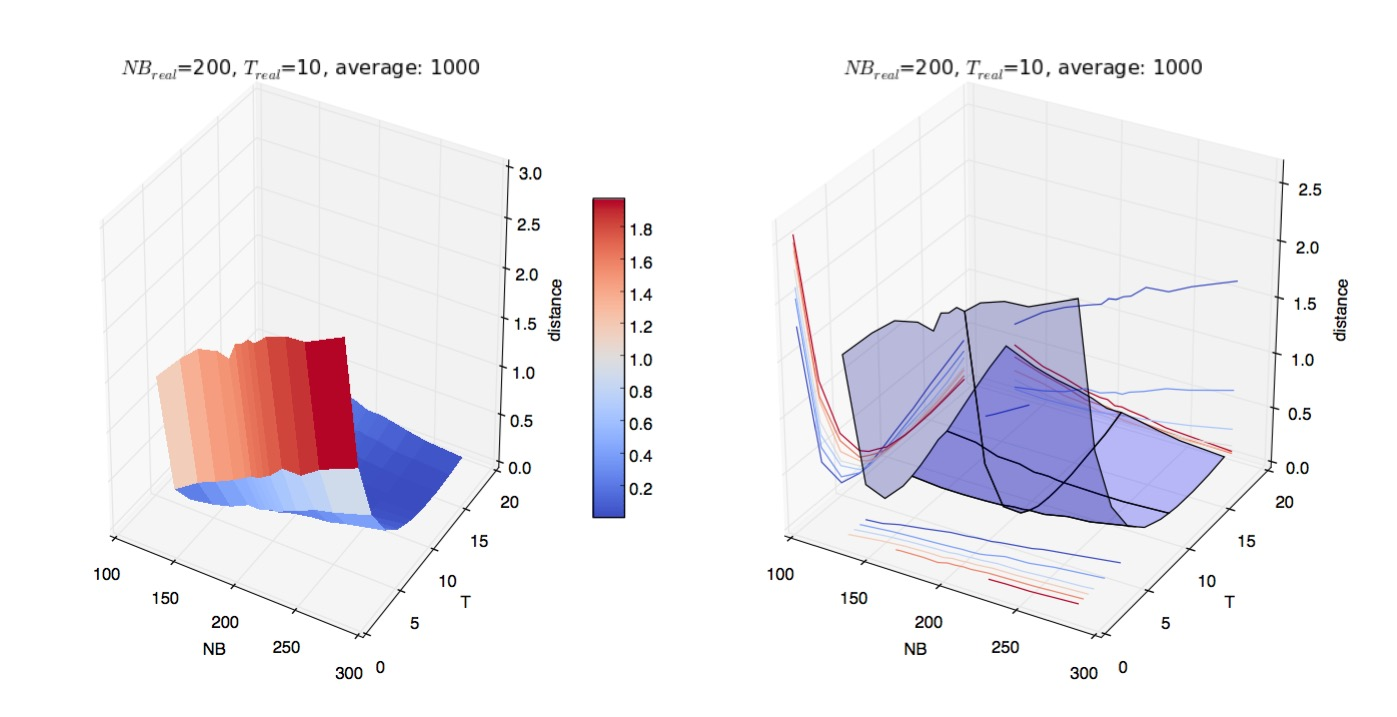
\includegraphics[width=270pt, height=150pt]{like_NBT.jpg}}
\caption{The joint distance surface for $T$ and $TB$ if true parameter is $T=10,TB=30$. It seems that the ratio of this two parameters matters in minimizing the distance.}\label{fig:dis_NBT}
\end{figure}

We now try to evaluate whether or not the ratio of $NB$ and $T$, say $\frac{T}{NB}$, is feasible to be estimated. We set $T$ to different values, for example, $5$, $10$ and $20$ ($10$ is not shown below), and we try to draw the joint distance surface of $NB$ and $TB$, to check whether the ratio of $\frac{T}{NB}$ can be retrieved with different values of $T$. Figure~\ref{fig:dis_NBTBT5} and~\ref{fig:dis_NBTBT20} show more details. The results here are not very promising, for the two following points. So the new statistic does not show big improvement till now.

\begin{enumerate}
\item The estimation of $\frac{T}{NB}$ ($NB$ in practical evaluation) seems feasible, but greatly biased by the value of $TB$; such estimation is indeed better than the estimation with the old IBD segment number distribution statistic, which we will discuss later;
\item The joint estimation of $TB$ in this case is not feasible, but it's obviously feasible with the old statistic and we will also discuss it later
\end{enumerate}

\begin{figure}[h]
\centerline{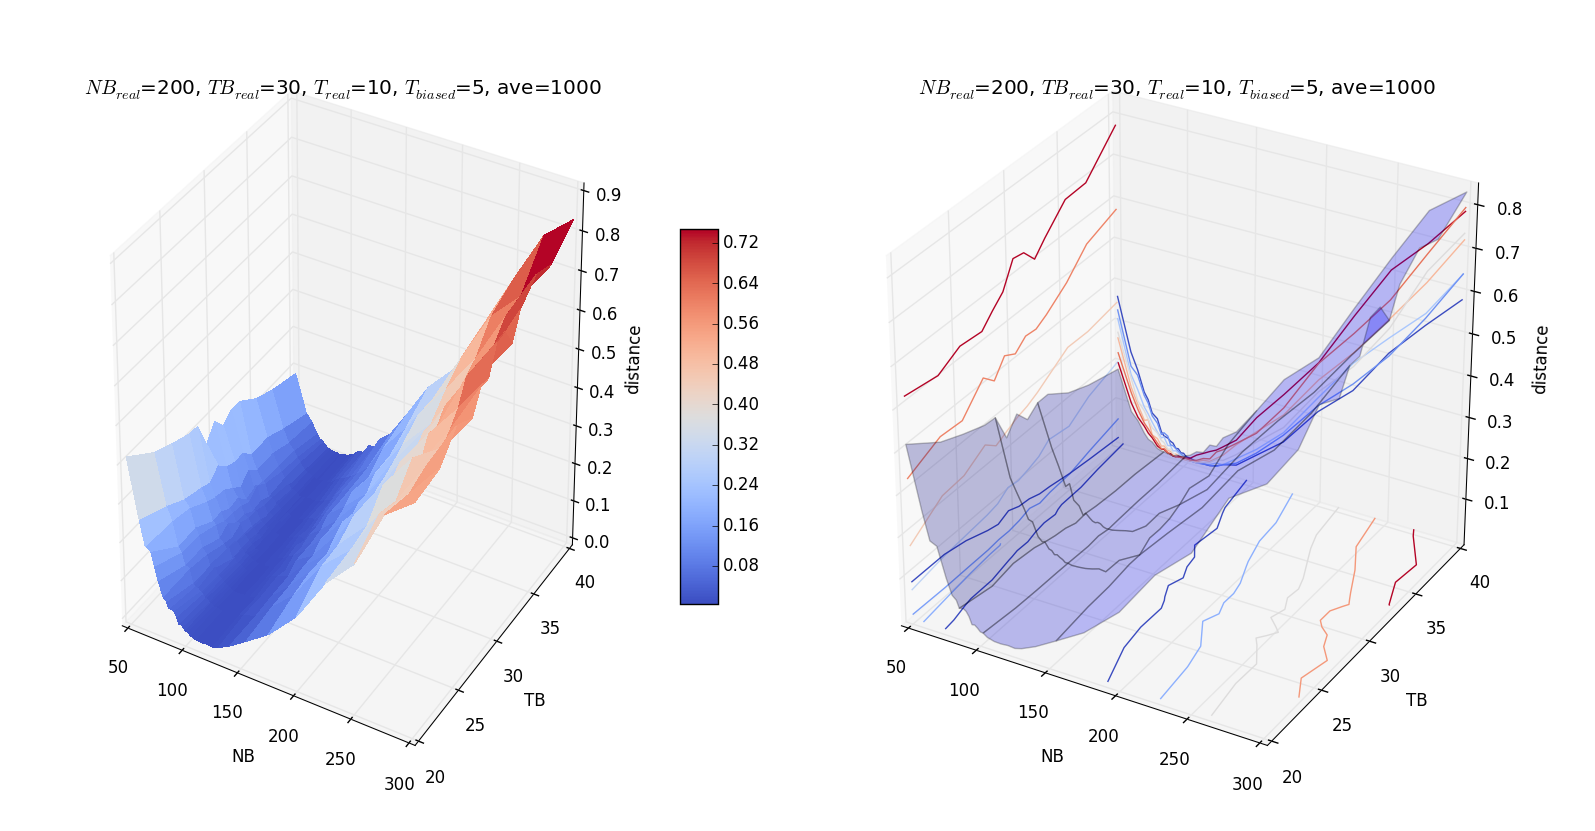
\includegraphics[width=270pt, height=150pt]{like_NBTBT5_2.png}}
\caption{The joint distance surface for $NB$ and $TB$ if true parameter is $NB=100$ (assuming constant $\frac{T}{NB}$, and $T$ is set to $5$), $TB=30$. We can see from the surface that, $TB$-dimension is always noisy (not estimatable), while $NB$-dimension seems good but still biased a lot.}\label{fig:dis_NBTBT5}
\end{figure}

\begin{figure}[h]
\centerline{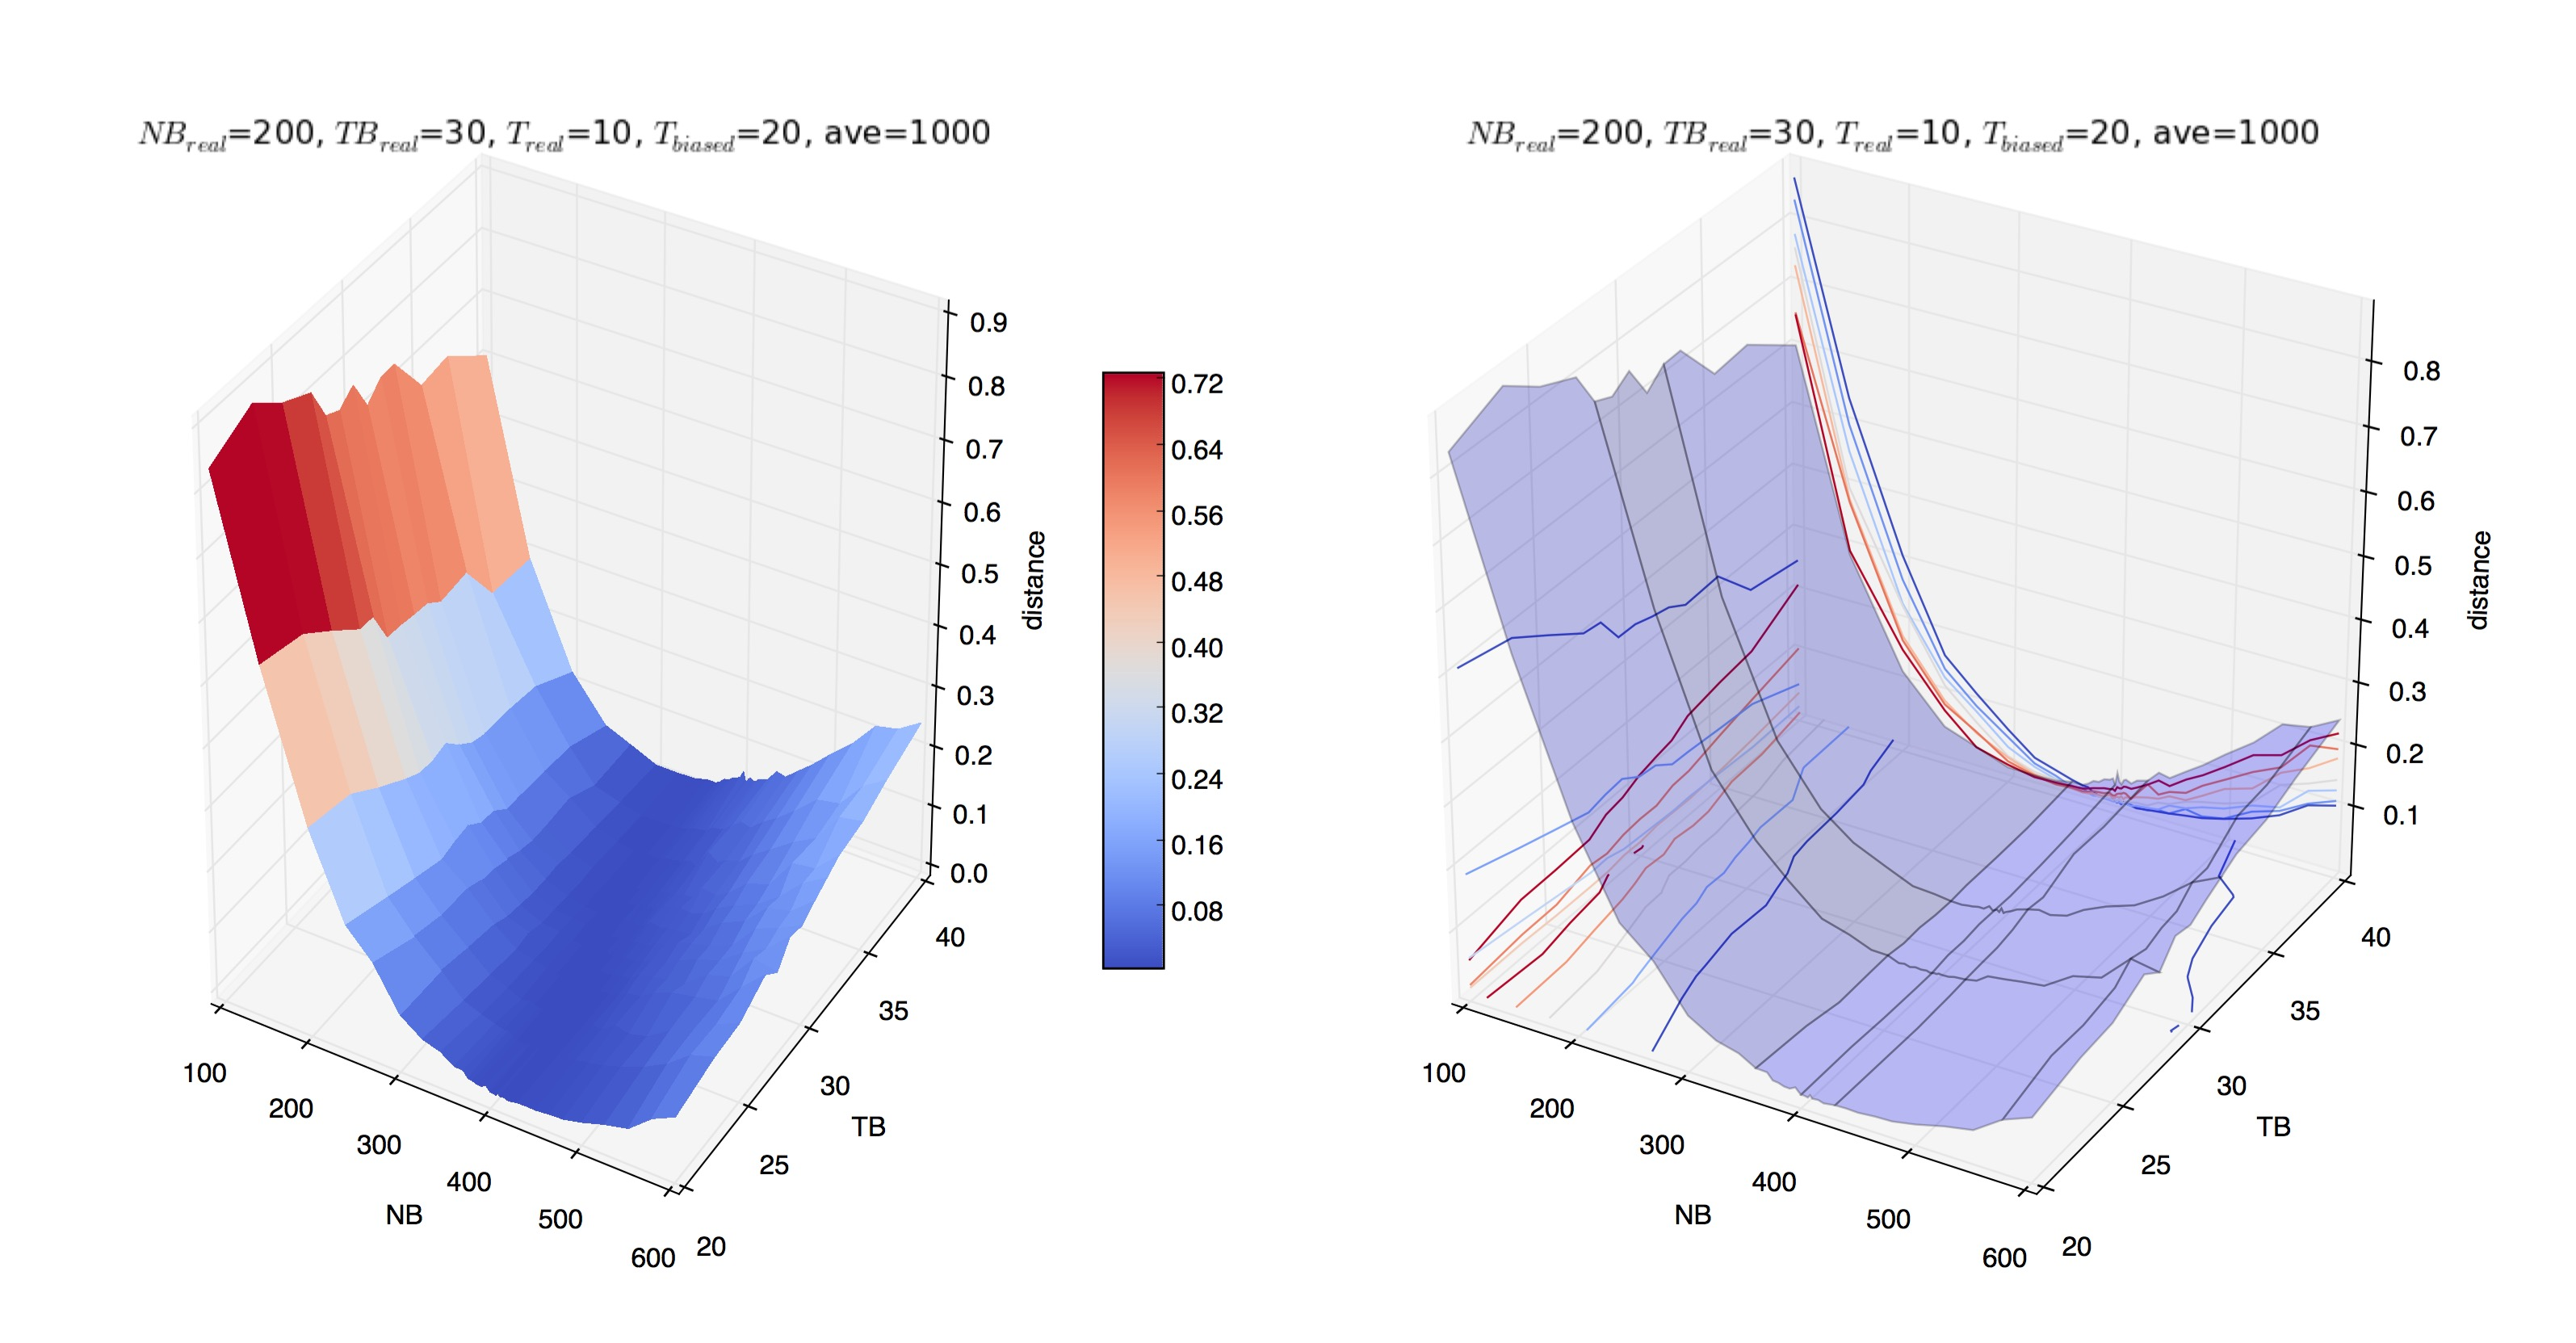
\includegraphics[width=270pt, height=150pt]{like_NBTBT20_2.jpg}}
\caption{The joint distance surface for $NB$ and $TB$ if true parameter is $NB=400$ (assuming constant $\frac{T}{NB}$, and $T$ is set to $20$), $TB=30$. We can see from the surface that, $TB$-dimension is always noisy (not estimatable), while $NB$-dimension seems good but still biased a lot.}\label{fig:dis_NBTBT20}
\end{figure}



\subsection{Combining statistics}

From above discussion, we find that all parameters here cannot be better estimated with the new statistic -- average IBD sharing statistic. We now try to combine the two statistics to see whether the combined statistic helps.

Here comes the idea of how to combine the two statistics and we try to let both of them contribute roughly equally to the combined statistic. We used the \textbf{Max} or \textbf{Mean} of the two statistics to normalize them first. For example, we let \textbf{Max}($distance\_curve_1$) $=x\times $ \textbf{Max}($distance\_curve_2$), where $x=0.4,0.7,1.0,1.3,1.6$. The same treatment was conducted for \textbf{Mean}. After normalization, we simply added the distance curves of the two statistics together, and check whether the results were smoother, or more convex. In reality, this combination doesn't help at all. And here we only use two simple examples for demonstration, $NA$ and $NC$, in Figure~\ref{fig:dis_com_NA} and Figure~\ref{fig:dis_com_NC}.

\begin{figure}[h]
\centerline{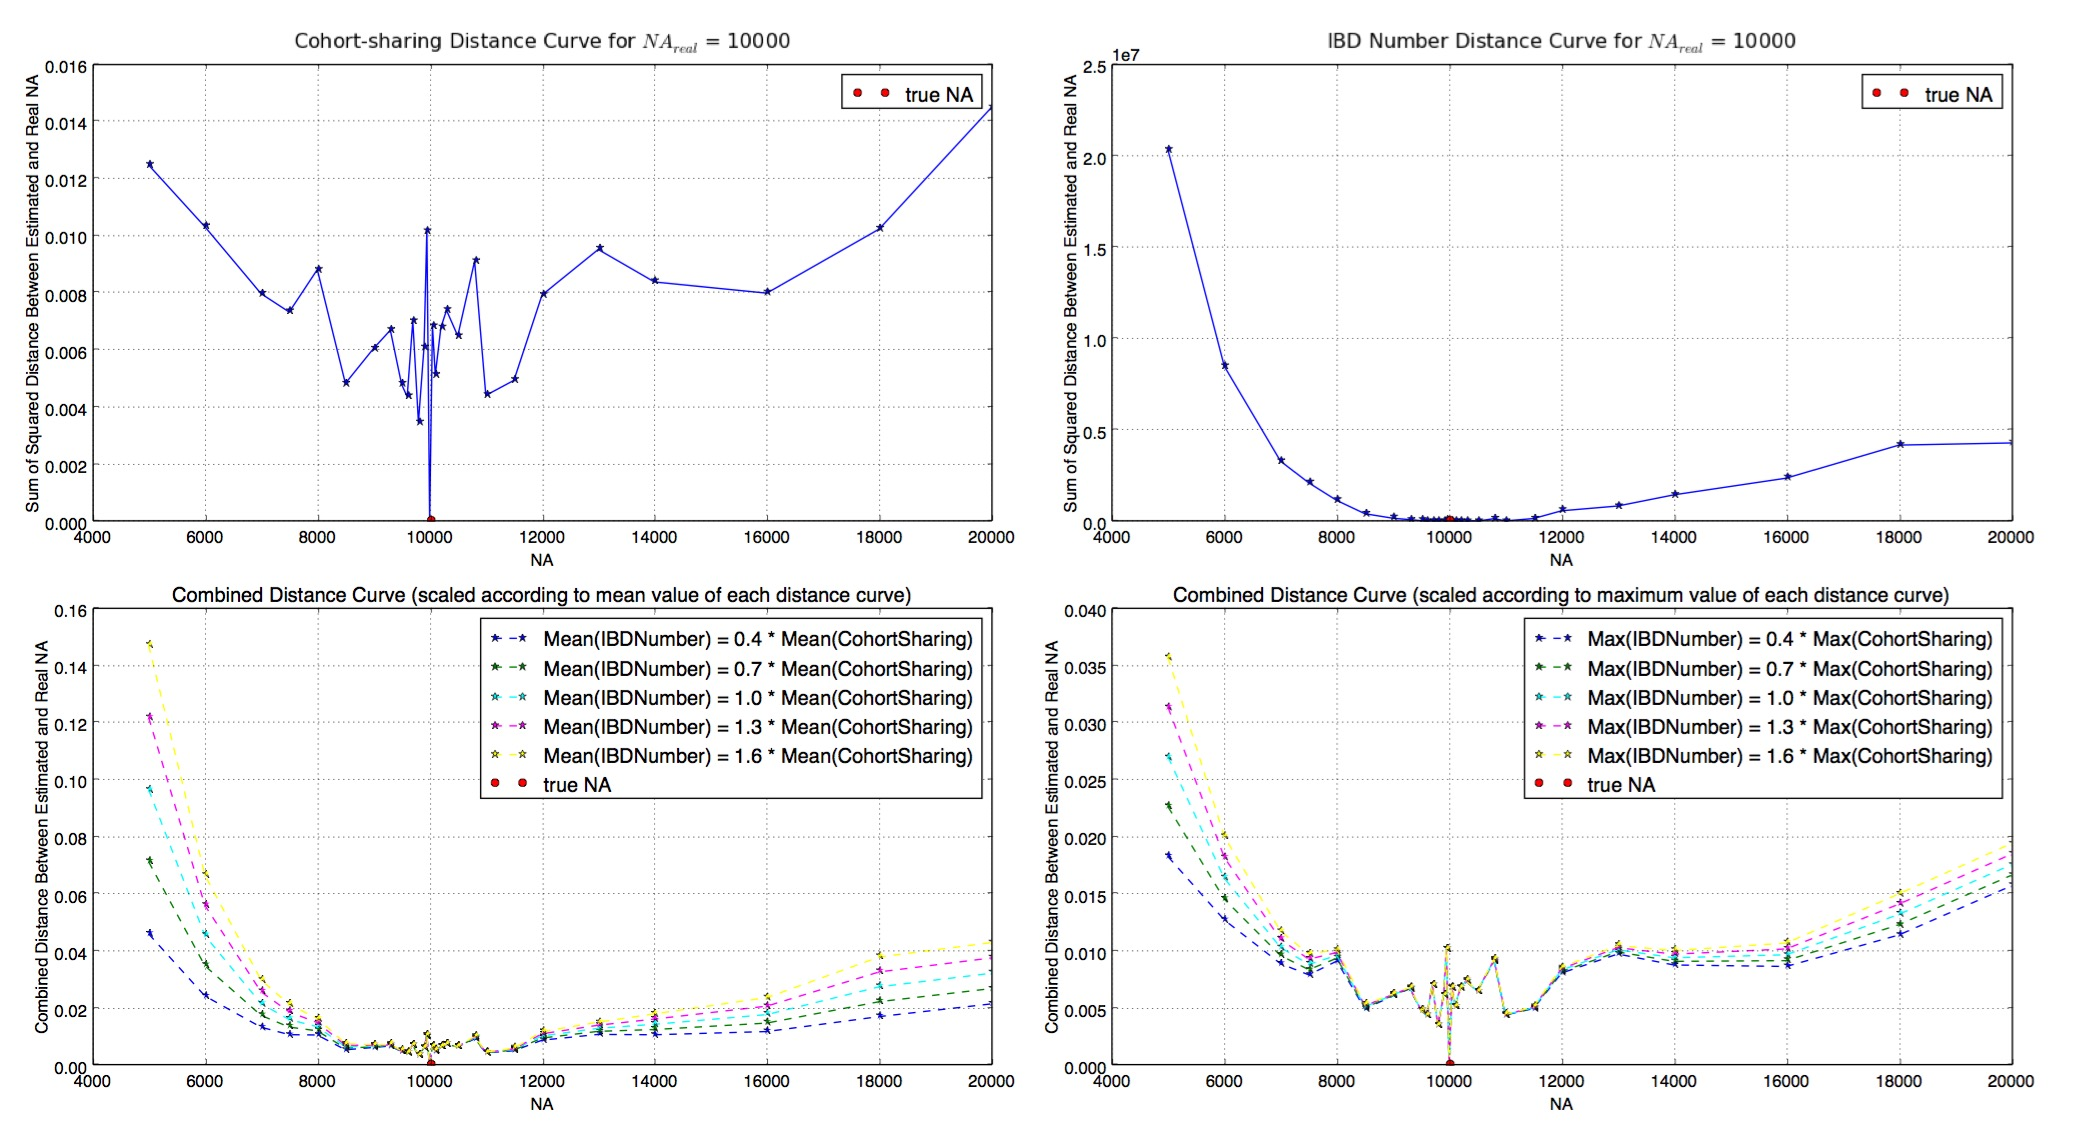
\includegraphics[width=280pt, height=170pt]{like_com_NA.jpg}}
\caption{Distance curves for $NA$. The above two curves are the distance curve for average IBD sharing and IBD segment number distribution, and the below two curves are the combined curve according to \textbf{Mean} value and \textbf{Max} value, respectively.}\label{fig:dis_com_NA}
\end{figure}

\begin{figure}[h]
\centerline{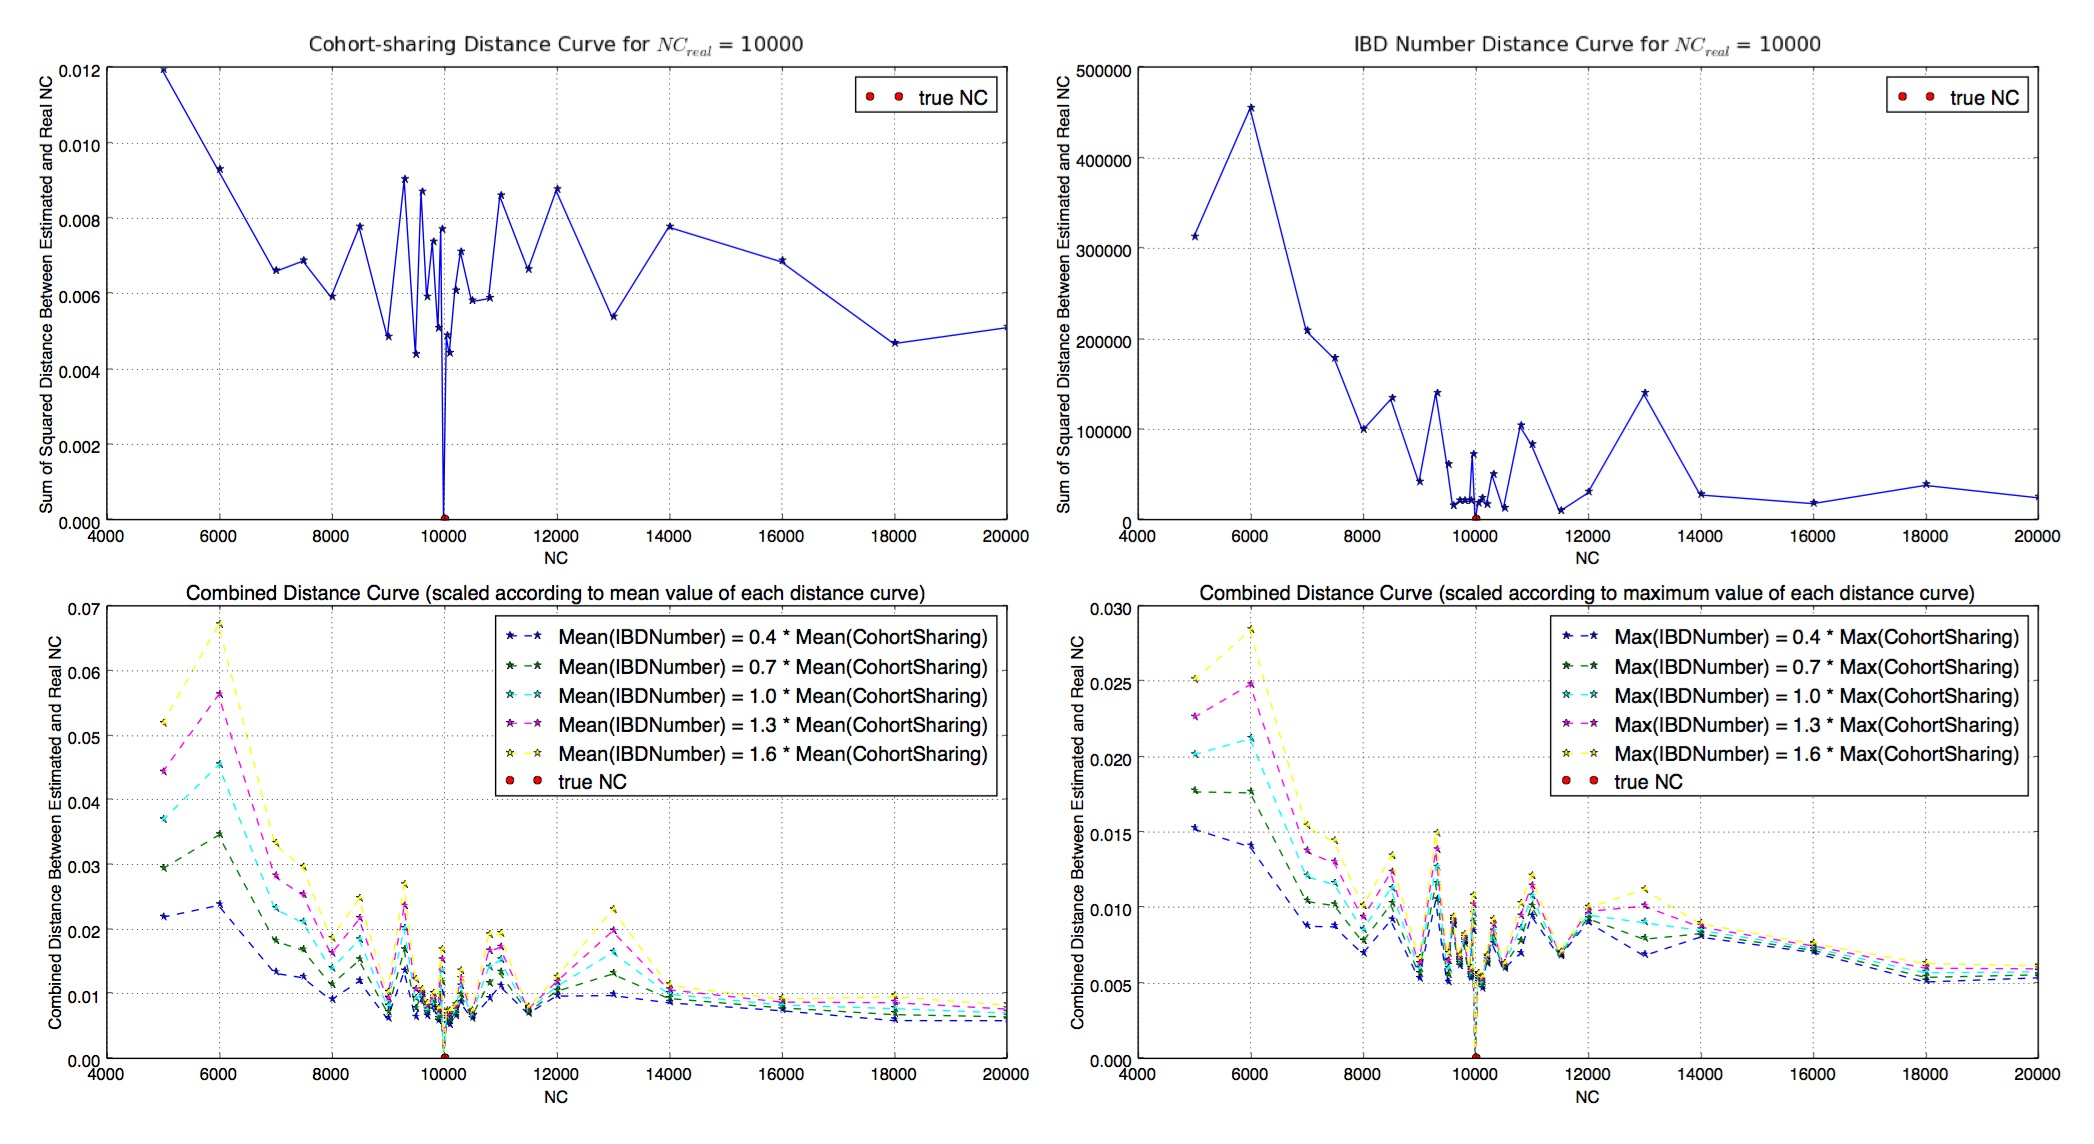
\includegraphics[width=280pt, height=170pt]{like_com_NC.jpg}}
\caption{Distance curves for $NC$. The above two curves are the distance curve for average IBD sharing and IBD segment number distribution, and the below two curves are the combined curve according to \textbf{Mean} value and \textbf{Max} value, respectively.}\label{fig:dis_com_NC}
\end{figure}



\section{Discussion}

The new statistic actually doesn't flash out in our inference framework. Also, the combination of the new statistic with the old IBD number distribution won't help in our inference framework either.

In the constant population size model, the average IBD sharing statistic is indeed a good indicator of the true population size. However, our old statistic (IBD segment number distribution) can also estimate the true population size. In one word, the new statistic doesn't beat the old one.

In the bottleneck population size model, the new statistic is not better than the old statistic, either. We have the following parameters to be evaluated in this bottleneck model:

\begin{enumerate}
\item $NA$: ancient population size;
\item $NC$: current population size;
\item $TB$: time to bottleneck event;
\item $NB$: bottleneck population size; or $T$: bottleneck duration;
\item $\frac{T}{NB}$: bottleneck strength
\end{enumerate}

In the figures and analysis shown in the previous sections and in this section, we don't show all the old results, but our comparison does use some observations from the old statistic. For $NA$ or $NC$, the old and the new statistics both can't determine the true value, as the distance curves are neither convex nor smooth. For $TB$, the new statistic is not able to indicate the true parameter, while the old statistic can. For $NB$ or $T$, if all other parameters are set to their true value, the old and the new statistics show the same performance, and for both the new and old statistics, these two parameters can always be retrieved even with imperfect information of $TB$. For the bottleneck strength $\frac{T}{NB}$, the results from the new statistic will be biased by the value of $TB$, while the results from the old statistic will not, but rather they can always be precisely estimated (See Figure~\ref{fig:TNBTB_old}). So, over all, the new statistic doesn't perform better than the old one, although it shows the same trend for some parameters explored.

\begin{figure}[h]
\centerline{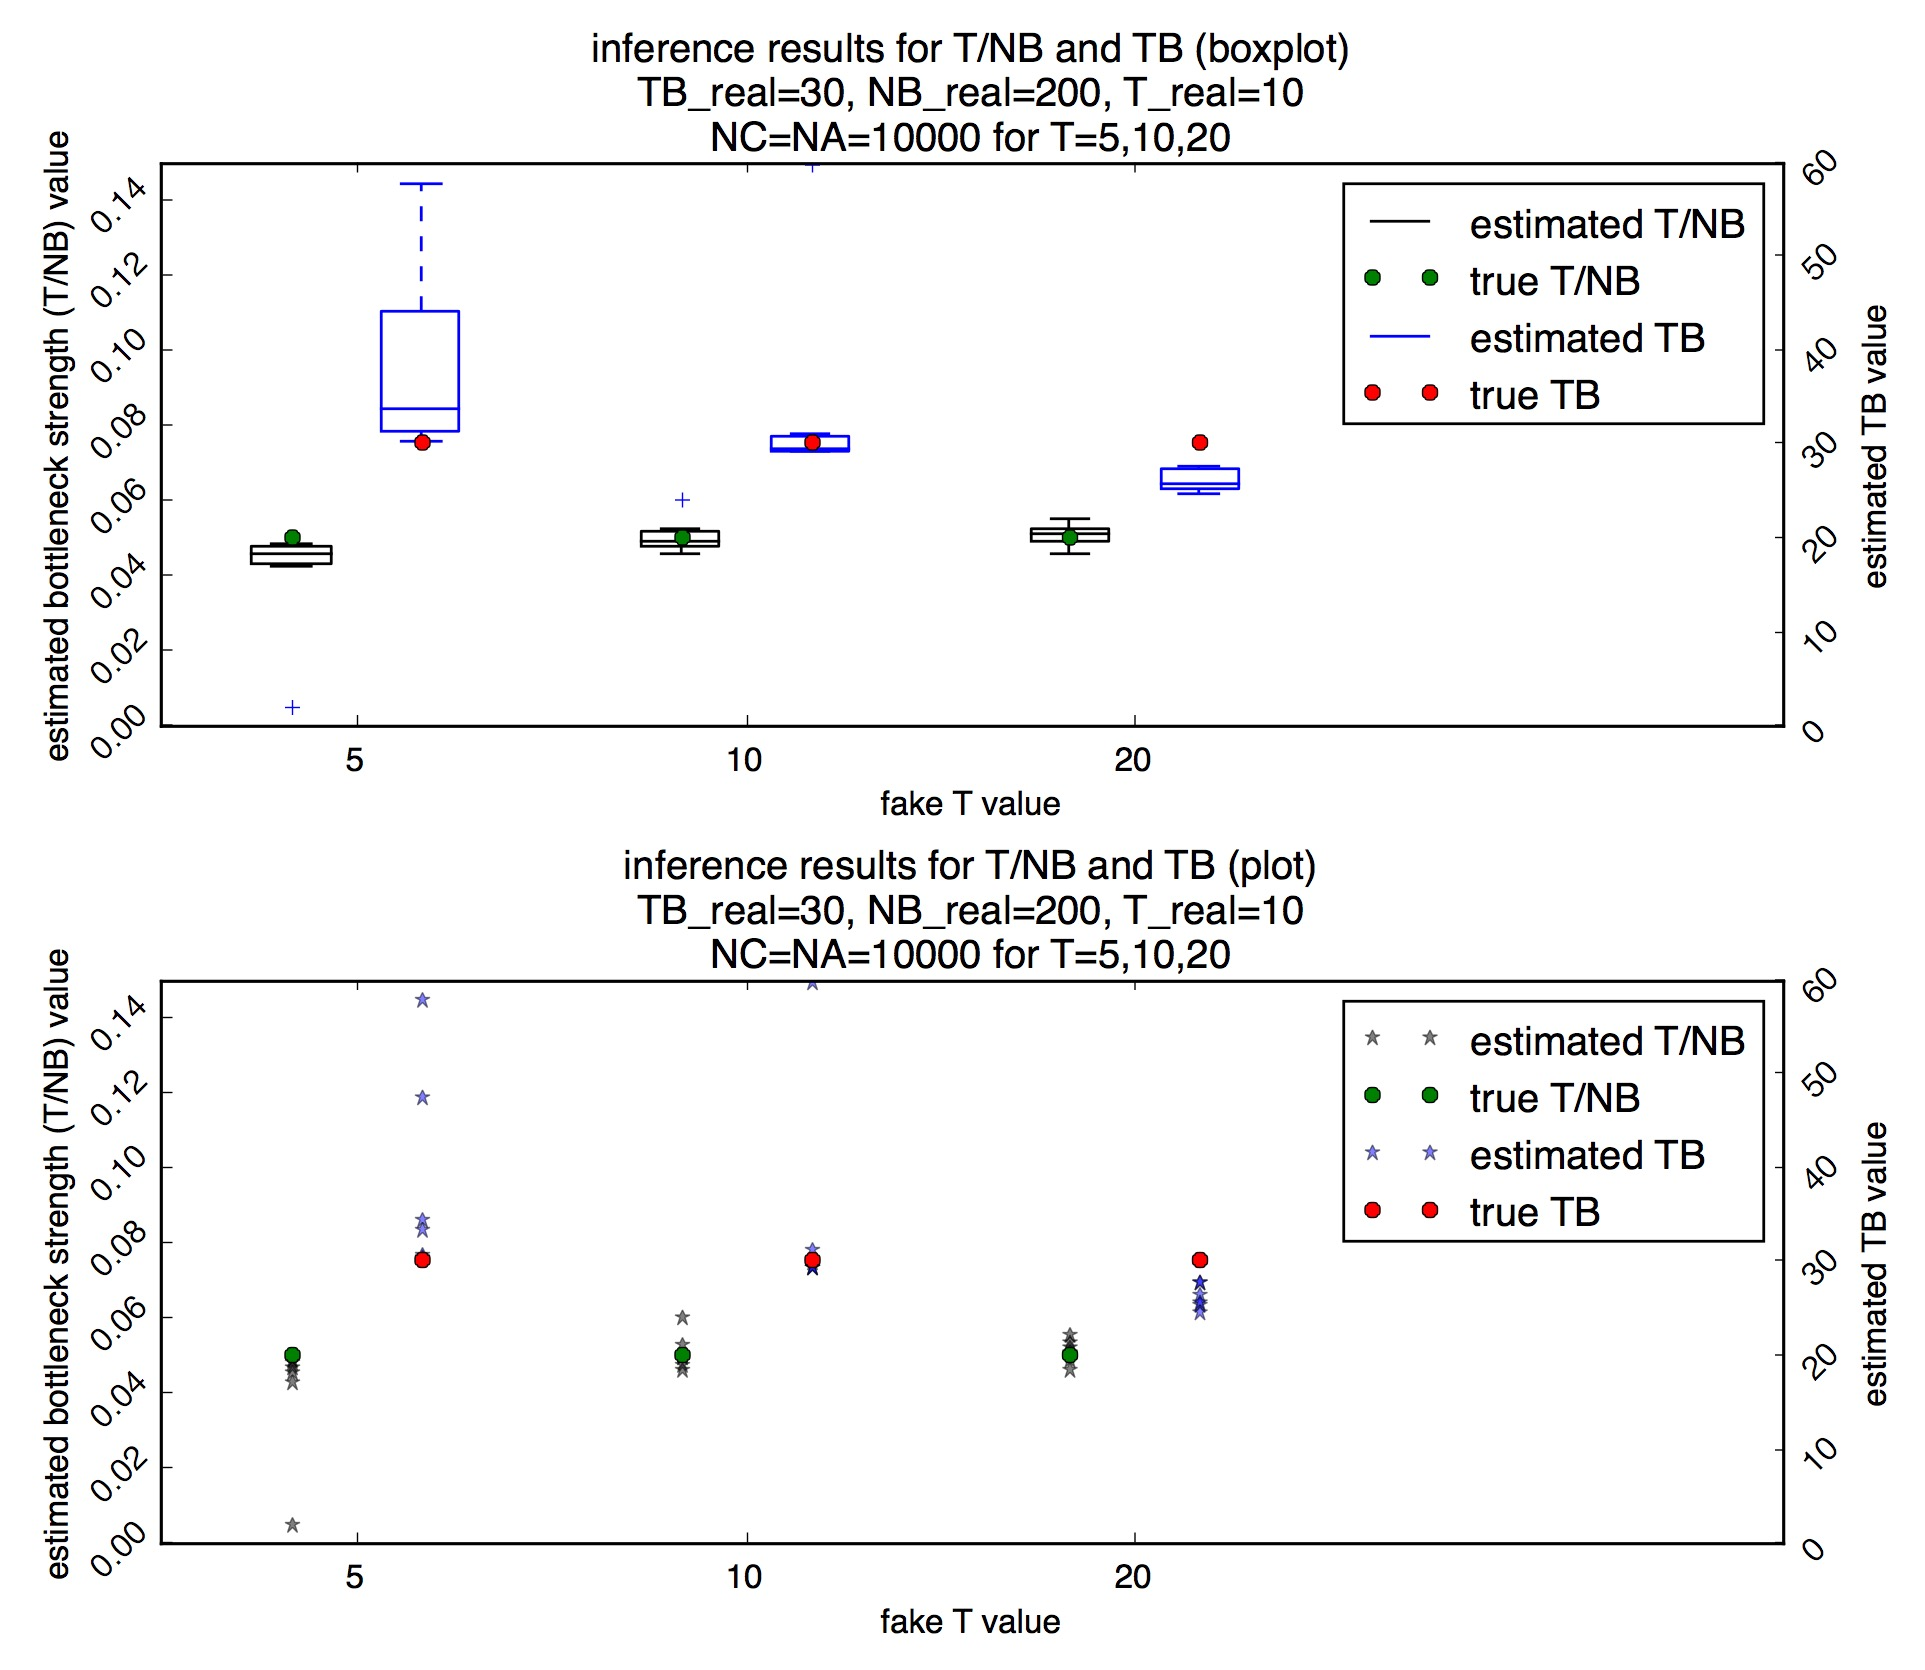
\includegraphics[width=250pt, height=210pt]{TNBTB_old.jpg}}
\caption{Estimation (old results) for $\frac{T}{NB}$ and $TB$ jointly, expressed in boxplot and plot format. We can see that, the estimation of $\frac{T}{NB}$ is always good, unbiased with $TB$. At the same time, the estimation of $TB$ jointly is feasible, though a little biased by the chosen value of $T$.}\label{fig:TNBTB_old}
\end{figure}

From the results, we find that combining the two statistics won't help either. In conclusion the new statistic doesn't improve the performance of the demographic inference we use.





\section{Conclusion}

In this project, we did extensive simulations to evaluate average IBD sharing statistic used in demographic inference, via minimum-distance method. This new statistic doesn't perform better than the old one with IBD number distribution statistic, as we discussed in the previous sections. And combining the new statistic with the old one won't improve the precision of the inference either. However, as this project is basically evaluation-oriented, we have already completed our original goal.

We wish that in the future, we could have a more gentle start for a scientific project, with solid scientific intuition and motivation. Otherwise, it may not be exciting enough, as simple hypothesis seldom turns out to be correct in scientific research. We also should not reply too much on simulation-based approach, especially use it as the main research approach. Simulation is more appropriate for evaluating the existing theories, instead of substituting them. For these reasons, out accomplishment is not as satisfactory as we expected.






\section*{Acknowledgement}

We thank Dr. Shai Carmi, the course instructor Prof. Itsik Pe'er of COMS4761 and TA Mr. Cameron Palmer for the helpful advices and discussions for this project. We also thank the feedback from the classmates during the project presentation sections.


\paragraph{Funding\textcolon} This is a course project in Columbia University Computer Science, and no
direct funding is issued.



\bibliographystyle{natbib}
%\bibliographystyle{achemnat}
%\bibliographystyle{plainnat}
%\bibliographystyle{abbrv}
%\bibliographystyle{bioinformatics}
%\bibliographystyle{plain}
\bibliography{document.bib}



\end{document}




% something else:
% table:
%\begin{table}[!t]
%\processtable{This is table caption\label{Tab:01}}
%{\begin{tabular}{llll}\toprule
%head1 & head2 & head3 & head4\\\midrule
%row1 & row1 & row1 & row1\\
%row2 & row2 & row2 & row2\\
%row3 & row3 & row3 & row3\\
%row4 & row4 & row4 & row4\\\botrule
%\end{tabular}}{This is a footnote}
%\end{table}

% equation:
%\begin{equation}
%\sum x+ y =Z\label{eq:01}
%\end{equation}